\section{Interface Design}
\label{sec:sm-design}

\subsection{Approach}
In the initial design session of the workshops, we considered all elicited requirements and agreed that SenseMap needs to:
\begin{enumerate}
	\item Capture web pages that the user visited, the sensemaking actions that happened there, and how the user arrived at those pages.
	\item Visualize the captured information in such a way that the user can understand what they have done, how things are connected, and what else they may do next.
	\item Support the user to curate the collected information according to its relevance, facilitate their reasoning, and communicate the findings. Also, this should not interfere with the original relationship among collected information so that the user can always use it as a reference.
\end{enumerate}

\subsection{Overview}
SenseMap consists of three views:

\begin{itemize}
	\item A \textit{Browser View} (\autoref{fig:sm-overview}A) that is a standard web browser with additional sensemaking support and provenance capture of actions happening there.
	\item A \emph{History Map} (\autoref{fig:sm-overview}B) that shows captured sensemaking actions with their page linking provenance while preserving their temporal order as much as possible to provide an overview of the sensemaking process (Point 2 above).
	\item A \emph{Knowledge Map} (\autoref{fig:sm-overview}C) that allows users to curate the collected information. This map is separate from History Map to preserve the semantic and temporal structure of the captured information (Point 3 above).
\end{itemize}

\begin{figure}[!htb]
 	\centering
 	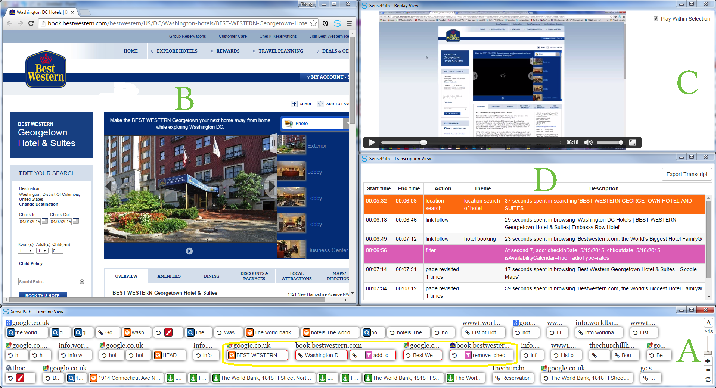
\includegraphics[width=\linewidth]{overview}
 	\caption[Three linked views of SenseMap]{Three linked views of SenseMap. \textbf{A:} This is the standard browser with additional sensemaking and provenance support. \textbf{B:} The history map captures and visualizes user actions to provide an overview of the sensemaking process. \textbf{C:} The knowledge map enables users to curate and make sense of the most relevant information to their tasks.}
 	\label{fig:sm-overview}
\end{figure}

In the next three sections, we will discuss these views and how they address the design requirements. \autoref{fig:view-and-process} summarizes the support that each view provides.

\begin{figure}[!htb]
	\centering
	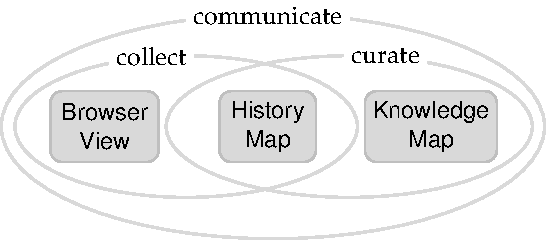
\includegraphics{view-and-process}
	\caption[Views and the sensemaking subprocesses they support]{Views and the sensemaking subprocesses they support. \emph{Collection} is supported in Browser View and History Map. \emph{Curation} is supported in History Map and Knowledge Map. \emph{Communication} is supported in all three views.}
	\label{fig:view-and-process}
\end{figure}

\subsection{Browser View}
This is a standard web browser with provenance capture and additional sensemaking support. The content and method to capture such provenance is the same as in the previous chapter, \autoref{sub:sp-provenance}. Additional features augmented to the browser are described as follows.

Highlighting and annotation are essential editing support. They allow users to mark relevant information and to assign their own interpretation (Requirement 4). A new option ``Highlight'' is added to the context menu when a passage of text is selected allowing the user to highlight it. That text becomes clickable allowing the user to either write a note or remove the highlight.

When a web page is visited, SenseMap takes a screenshot and uses it to represent the page in the history map (\autoref{sub:collection}). It is intended to help the user to quickly recognize web pages that have been visited (Requirement 2). However, that screenshot may not reflect perfectly the main content of the web page, especially when the picture contains lots of text. To address this issue, we allow the user to assign a custom representative image to a web page. This can be done by simply right-clicking on any images in the web page and select ``Set as Page Image'' option in the context menu.

\subsection{History Map}
\label{sub:collection}
This map provides an overview of the sensemaking process using the captured actions and their provenance (\autoref{fig:sm-overview}B).

\subsubsection{Visual Representation}
An action is represented as a bar with an icon indicating its type and text showing the contextual information. Icons help users to recognize action types faster and we use the same icon set as shown in the previous chapter, \autoref{fig:icon-list}. If the action type is the default \textit{browsing}, the favorite icon of its web page is used instead. The contextual text is important to understand what the action is about and it is truncated up to a certain length to fit to the limited space. \autoref{fig:action-bar} shows an example of a keyword search action.

\begin{figure}[!htb]
	\centering
	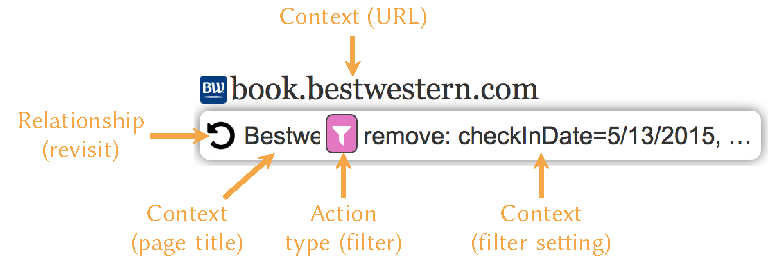
\includegraphics[width=.3\linewidth]{action-bar}
	\caption{Action bar for a keyword search ``visual analytics conference''.}
	\label{fig:action-bar}
\end{figure}

Highlights and annotations of the same web page are grouped together as in \autoref{fig:action-highlights}. They are located in separate rows below the web page title. By default, just a few highlights and annotations are shown to ensure a reasonable height for the page. All of them can be revealed using a menu available when hovering on any highlight or annotation.

\begin{figure}[!htb]
	\centering
	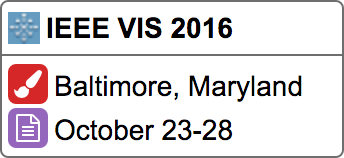
\includegraphics[width=.3\linewidth]{action-highlights}
	\caption{A page with one highlight and one note.}
	\label{fig:action-highlights}
\end{figure}

To provide a connection between the history map and the browser view, the action bar corresponding to the active browser tab is highlighted in cyan. Pages that have been opened but have not seen yet (could be the result of opening links in new tabs) are shown with a dashed border, which may help to remind the user on reading them. \autoref{fig:action-active-not-seen} shows an example of pages with these two states.

\begin{figure}[!htb]
	\centering
	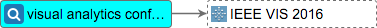
\includegraphics[width=.6\linewidth]{action-active-not-seen}
	\caption[Representation of active page]{The user is active on a search result page (left bar) and opens a link in a new tab (right bar).}
	\label{fig:action-active-not-seen}
\end{figure}

\subsubsection{Layout}
\label{sub:sm-layout}
Seeing the provenance of a web page is important to the user (Requirement 1). Currently, it can only be seen if the user presses and holds the browser's back button. This provenance information is not even available if a page is open in a new tab. In the history map, linking relationships between two pages are always visible and illustrated by an arrow pointing from the source to the target (\autoref{fig:action-active-not-seen}). For example, if the user clicks on a link in page $A$ yielding to page $B$, an arrow from $A$ to $B$ will be added to show this relationship. Showing links between pages can reveal branching structures such as when multiple pages are opened in new tabs from the search result page. This provides richer provenance information and easier access for the user compared to a linear list of visited pages as in current browsers.

Technically, all pages and links in the history map form a \textit{forest}, where tree roots are pages that do not have a parent page such as pages opened by entering the URLs manually. Temporal information of sibling pages are indicated by the order of them: earlier opened pages are placed above later ones. This also helps maintain the mental model for the user about their process: the order of pages are never changed; and a new page is added either on the right side of the page triggering its opening or at the bottom of the map when such linking does not exist. A virtual node is then added and connected to all tree roots to form a single tree. We use the compacted tree layout in \textit{jgraph} library~\footnote{\url{https://www.jgraph.com/}} to produce the location of pages (\autoref{fig:sm-overview}B).

Temporal information shows the order of actions that the user has taken, and the branching and linking relationships reveal their semantics. At a lower level, highlighting the active tab in the layout as described earlier helps the user know where the page they focusing (active) page in the context of the overall process. Both of these supports address Requirement 3.

\subsubsection{Preparation for Curation}
The history map displays all captured actions; however, probably not all of them are equally important and relevant to the sensemaking task. Therefore, it is necessary to allow users to assess the relevance of the collected information. We use the term \textit{node} to refer to either a simple search action bar or a page containing many highlights -- a node in the tree layout. Three levels of relevance are provided, all through the menu available when hovering a node.

\begin{enumerate}
	\item If a node is completely irrelevant, the user can \textit{remove} it.
	\item If a node is not quite relevant but the user wants to keep it to have a look at some point, they can \textit{minimize} it.
	\item If a node is very relevant, the user can \textit{favorite} it.
\end{enumerate}

When a node is removed, it and its links are removed from the map. When a node is minimized, it is collapsed into a small circle. This enables users to focus on other nodes and also save the display space. Favorite nodes are displayed with a yellow background and a thumbnail of the captured screenshot to increase their recognizability. \autoref{fig:action-minimize-favorite} shows an example of minimized and favorite nodes.

\begin{figure}[!htb]
	\centering
	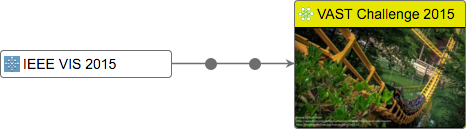
\includegraphics[width=.75\linewidth]{action-minimize-favorite}
	\caption[Pre-curated nodes]{Nodes are pre-curated: two irrelevant nodes in the middle are minimized, whereas the last one is set favorite.}
	\label{fig:action-minimize-favorite}
\end{figure}

\subsubsection{Scalability}
Nodes can reduce their size through zooming to accommodate more nodes within the visible part of the history map. By default, all nodes have the same width and the same maximum height, which allows a few words of the contextual text visible, and a reasonably large thumbnail image, which may help users recognize the visited pages. For each smaller level, both the node width and the number of highlights are reduced. The node height is adjusted so that the ratio between it and the node width remains unchanged. At the smallest level, only the action type icon or a small thumbnail image is shown. \autoref{fig:zoom} shows an example of different zoom levels applied onto the same node.

\begin{figure}[!htb]
	\centering
	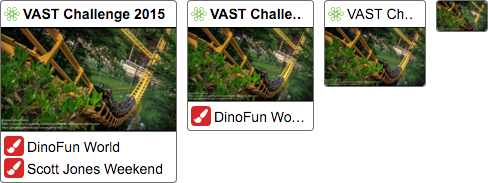
\includegraphics[width=.85\linewidth]{zoom}
	\caption{The same node with four zoom levels.}
	\label{fig:zoom}
\end{figure}

Node zoom level is explicitly controlled by the user using simple plus/minus buttons. When the collection of nodes exceeds the visible area, the user can pan the map to see them.

\subsubsection{Revisitation and Interruption}
When an action is captured, its web page's URL is also recorded. Clicking on a node opens its associated web page. This releases the user from worrying about losing browser tabs. Moreover, the additional branching and linking structure of the layout could help the user find information faster than the linear list of page titles in the History feature of the standard web browsers (Requirement 2).

To provide a more fine-grained bookmarking and navigation than the web page URL level, revisiting a captured highlight brings the user to the exact text being highlighted. This is made possible by capturing the relative location of the highlight with respect to the root of the web page.

In the real world environment, the user may have many sensemaking tasks happening at the same time (Requirement 5). Even while working in a single task, the user may do some other things irrelevant to the task such as checking email and social feeds. Therefore, always capturing user actions and putting them into a single place will result a huge mix of unrelated information. To address this issue, we allow the user to create separate collections of information for different tasks. The user can also pause the information capture and resume when needed.

\subsection{Knowledge Map}
This map allows users to curate the information displayed in the history map (\autoref{fig:sm-overview}C).

\subsubsection{Visual Representation}
The curation process starts by adding nodes from the history map to the knowledge map. This is done via the \textit{Curate} button in the menu available when hovering over a node. Nodes in the knowledge map have the same visual representation with those in the history map. The only difference is that thumbnail images of curated nodes are always made visible to improve their recognizability (Requirement 6).

\subsubsection{Spatial Organization}
The limit of single dimensional ordering tabs from left to right is addressed in the knowledge map through the spatial organization of nodes (Requirement 7). The user can freely move nodes by simply dragging them around. This enables the user to spatially group nodes and to assign different meanings to them. \autoref{fig:free-movement} shows an example of a knowledge map with three clear groups based on their locations.

\begin{figure}[!htb]
	\centering
	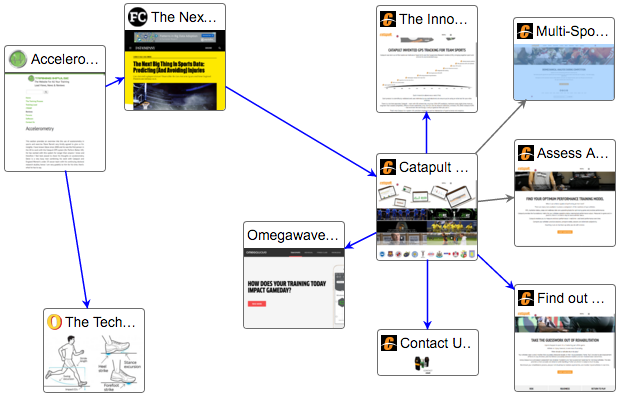
\includegraphics[width=\linewidth]{free-movement}
	\caption[An example of knowledge map]{A knowledge map with three clear groups of nodes as the result of free movement.}
	\label{fig:free-movement}
\end{figure}

\subsubsection{Linking/Unlinking}
Besides spatial grouping, seeing the casual relationships between collected information is also important to users in supporting sensemaking (Requirement 7). A conventional representation is used to show this relationship: an arrow pointing from the cause to the effect. The user can add a casual relationship by clicking on the ``cause node'', holding it for half a second until the cursor changes to an arrow, then  releasing the mouse on the ``effect node''.

When nodes are added to the history map, the provenance links among them are also copied to the knowledge map to provide an initial understanding of existing relations. Different colors are used to distinguish user-added links from provenance links.

\subsubsection{Formal Reasoning}
Currently, SenseMap does not support any formal argumentation methods. However, the flexibility of spatial organization and relationships establishment could help the user apply their reasoning strategies~\cite{Sedig2013}. For instance, users can draw a link from a ``hypothesis'' node to its evidence. Then, they can move all supporting evidence nodes to one area and all counter evidence nodes to a different location to distinguish the two groups.

\subsubsection{Collection -- Curation}
All nodes in the knowledge map appear in the history map, but the other direction is not always true because only relevant and important nodes may be curated. To help the user quickly recognize which nodes in the history map are already curated, a green ``tick'' icon is superimposed at the top right hand corner. Also, hovering a node in one map will highlight that node, if it exists, in the other map.

\subsection{Communication}
The final organization of curated information provides a complete picture of the sensemaking task, including the most important and relevant information to the users, which makes it ideal for them to present their findings (Requirement 11). If the process is of interest, the history map can be used alongside the knowledge map. Moreover, the user can refer to raw data, via node revisitation, to support their presentation (Requirement 12).

Both the history and knowledge maps can be saved as local files and loaded later. This allows users to share their maps (Requirement 14). Also, the user can create multiple copies of knowledge maps based on the same history map allowing customizing for various presentation purposes (Requirement 13).

\subsection{Implementation}
SenseMap is implemented as a Chrome extension based on the D3 visualization library~\cite{Bostock2011}. Chrome was chosen because of its high popularity. This decision was also confirmed in the initial interviews with seven out of nine participants using Chrome. Highlighting and annotation require modification of the web page structure, thus are implemented as content scripts using Chrome extension API. The provenance capture and action detection are implemented using the same method as in the previous chapter, \autoref{sub:sp-impl}.

%The three views communicate using \textit{messaging passing} mechanism provided by Chrome extension API. When an interaction occurs in one view, it sends a message to notify all other views. Each view constantly listens and responds to such messages.